In 1996, Ajtai discovered that there are mathematical problems in the area of lattices that have some desirable properties with respect to cryptography. Since then, lattices have been used to construct several
cryptosystems and other cryptographic applications. In this chapter, lattices are introduced and their connection with cryptography is examined.

\section{Lattice, definition and properties}
Lattice is a set of points in $n$-dimensional space with a periodic structure. More formally, given $n$-linearly independent vectors $\textbf{b}_1, \dots, \textbf{b}_n \in \mathbb{R}^n$, the lattice generated by them is the set of vectors:

\[\mathcal{L}(\textbf{b}_1, \dots, \textbf{b}_n) = \bigg\{\sum_{i=1}^{n} x_i \textbf{b}_i: x_i \in \mathbb{Z} \bigg\}\]

Linear independence means that no vector can be written as linear combination of the other vectors. The set of vectors $\{\textbf{b}_1, \dots , \textbf{b}_n\}$ are known as a basis of the lattice. Below are fundamental properties of lattices:

% Lattice in $\mathbb {R}^{n}$ is a subgroup of $\mathbb {R}^{n}$, and it spans the real vector space $\mathbb {R}^{n}$.

\textbf{Rank of lattice:}
The rank of a lattice is defined as the number of linearly independent vectors in any basis for that lattice. Full-rank lattice is defined as a lattice where the number of linearly independent vectors in any basis for this lattice is exactly equal to the number of dimensions in which the lattice is embedded. In such an instance, it is clear that any basis for such a lattice can be described by a set of $n$ vectors, each of $n$ dimensions. We can thus describe the basis as a square integer matrix.

\textbf{Determinant of lattice:}
Lattice determinants measures properties about the lattice. Specifically, $\det(\mathcal{L}_\textbf{B})$ is the $n$-dimensional volume of the fundamental parallelepiped defined by the lattice basis $\textbf{B}$. Since we will only be operating with full-rank lattices, we can simplify the definition of this lattice determinant as being the absolute value of the determinant of some basis of the lattice.

\begin{figure}[H]
	\centering
	$\det(\mathcal{L}_\textbf{B} ) = |\det(\textbf{B})|, \textbf{B} \in \mathbb{Z}^{n \times n}$
\end{figure}

\begin{definition}
\normalfont
The unimodular matrix is defined as an integer matrix, whose inverse is also integral. This implies the following properties: $\textbf{U}$ must be integral matrix, must be square matrix and $\det(\textbf{U})$ must be exactly $+1$ or $-1$.
\end{definition}

Any multiplication of a lattice basis with a unimodular matrix will produce a new basis that would generate the same lattice. This is due to the determinant of a unimodular matrix being $+1$ or $-1$. In fact, lattice equality is only achieved if there exists such a unimodular transform between bases. The determinant of a lattice is inverse proportional to its density: the smaller determinant, the denser the lattice would be.



\begin{figure}[H]
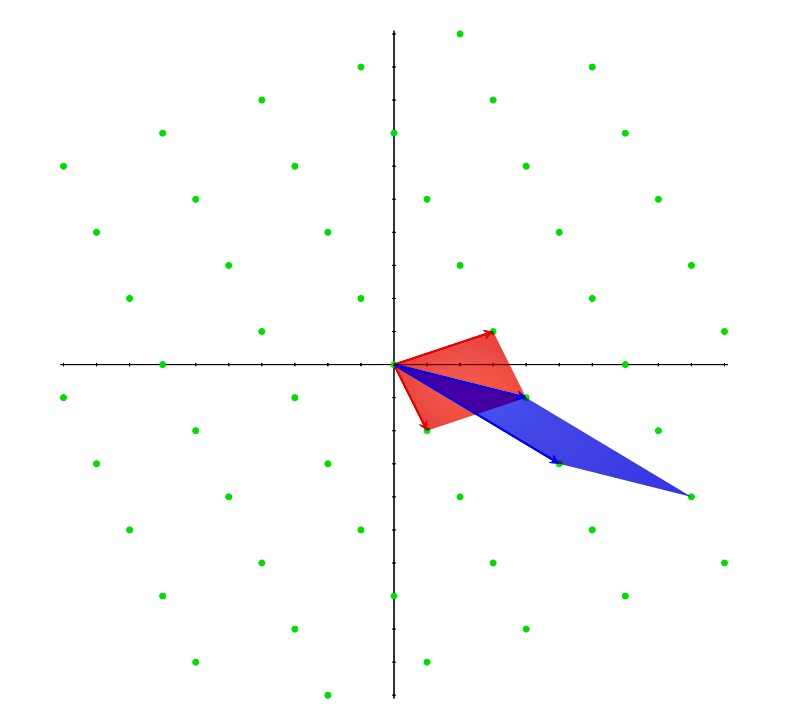
\includegraphics[scale=0.28]{lattice-two-region}
\centering
\caption{Two fundamental parallelepiped of the same lattice}
\figuresubtitle{The determinant of lattice is equal to the volume (i.e. area in $2$-dimensions) of fundamental parallelepiped.}
\end{figure}


\textbf{Hermite normal form: }
Various authors may prefer to talk about Hermite Normal Form in either row-style or column-style. They are essentially the same up to transposition.

\textit{(Row-style) Hermite Normal Form}: $m$ by $n$ matrix $\textbf{A}$ with integer entries has a (row) Hermite normal form ($\mathrm{HNF}$) $\textbf{H}$ if there is a square unimodular matrix $\textbf{U}$ where $\textbf{H}=\textbf{U} \times \textbf{A}$ and $\textbf{H}$ has the following restrictions:


\begin{enumerate}
    \item $\textbf{H}_{ij}=0$ for $j>i$,
    \item $\textbf{H}_{ii}>0$ for all $i$, and
    \item $\textbf{H}_{ij} \le 0$ and $|\textbf{H}_{ij}|<\textbf{H}_{ii}$ for $j<i$
\end{enumerate}




Note that the row-style definition has a unimodular matrix $\textbf{U}$ multiplying $\textbf{A}$ on the left (meaning $\textbf{U}$ is acting on the rows of $\textbf{A}$), while the column-style definition has the unimodular matrix action on the columns of $\textbf{A}$. The two definitions of Hermite normal forms are simply transposes of each other.

For every matrix, there exist a Hermite normal form and it is unique. In details, for every $m$ by $n$ matrix $\textbf{A}$ with integer entries has a unique $m$ by $n$ matrix $\textbf{H}$ ($\mathrm{HNF}$), such that $\textbf{H}=\textbf{U} \times \textbf{A}$ for some square unimodular matrix $\textbf{U}$.

Typical lattice in $\mathbb{R}^{n}$ has the form $\mathcal{L}=\left\{\left.\sum _{i=1}^{n}\alpha _{i}\textbf{a}_{i}\;\right\vert \;\alpha _{i}\in {\mathbb {Z}}\right\}$ where the $\textbf{a}_i$ are in $\mathbb{R}^n$. If the columns of a matrix $\textbf{A}$ are the $\textbf{a}_i$, the lattice can be associated with the columns of a matrix, and $\textbf{A}$ is said to be a basis of $\mathcal{L}$. Because the Hermite normal form is unique, it can be used to answer many questions about two lattice descriptions. For what follows, $\mathcal{L}_{\textbf{A}}$ denotes the lattice generated by the columns of $\textbf{A}$. Because the basis is in the columns of the matrix $\textbf{A}$, the column-style Hermite normal form must be used. Given two basis for a lattice, $\textbf{A}$ and $\textbf{A}'$, the equivalence problem is to decide if $\mathcal{L}_{\textbf{A}}=\mathcal{L}_{\textbf{A}'}$. This can be done by checking if the column-style Hermite normal form of $\textbf{A}$ and $\textbf{A}'$ are the same.



\textbf{Euclidean norm:} Many problems in lattice theory involve distance minimization. The most intuitive way to measure distance in a multi-dimensional space is by using the Euclidean norm ($l_2$). This norm comes from Pythagoras' theorem, stating that the distance between two points is the square root of the sum of the axial distances squared. This can be extended to an arbitrary, finite-dimensioned vector space by squaring each of the axial dimensions and taking the square root of the sum. Let $w$ be a vector of $\mathbb{R}^n$. The Euclidean norm is the function $||.||_2$ defined by: $||w||_2 = \sqrt{\sum_{i=1}^n{|w_i|^2}}$

\textbf{Successive minima:}
One basic parameter of a lattice is the length of the shortest nonzero vector in the lattice (we have to ask for a nonzero vector since the zero vector is always contained in a lattice and its norm is zero). This parameter is denoted by $\lambda_1$. An equivalent way to define $\lambda_1$ is the following: it is the smallest $r$ such that the lattice points inside a ball of radius $r$ span a space of dimension $1$. This definition leads to the generalization of $\lambda_1$, known as successive minima or $\lambda_i$; that is the smallest $r$ such that lattice points inside a ball of radius $r$ span a space of dimension $i$.


\begin{figure}[H]
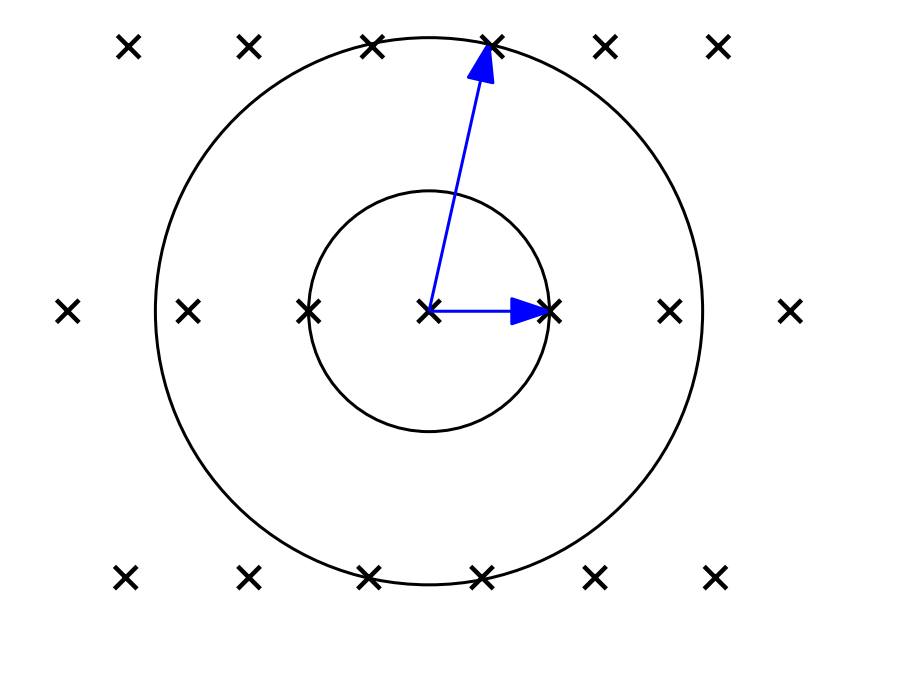
\includegraphics[scale=0.15]{minima}
\centering
\caption{Visualization of first and second lattice minima}
\figuresubtitle{$\lambda_1(\mathcal{L}) = 1, \lambda_2(\mathcal{L}) = 2.3$}
\end{figure} 

\subsection{Examples of lattices}
\begin{enumerate}
    \item Below shows the lattice in $2$ dimensions generated by the vectors $(1, 0)^t$ and $(0, 1)^t$. This lattice is the set of all points in $\mathbb{R}^2$ with integer coordinates. This can be generalized to $n$ dimensions, where the lattice $\mathbb{Z}^n$ is called the \textit{integer lattice}.
    
\begin{figure}[H]
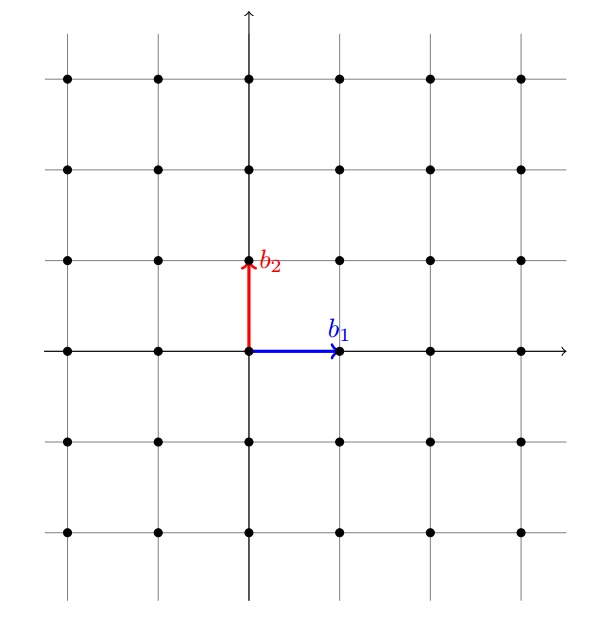
\includegraphics[scale=0.2]{lattices/1}
\centering
\caption{Lattice $\mathbb{Z}^n$ with basis vectors $(0, 1)^t$ and $(1, 0)^t$}
\end{figure}    
    
    \item Below shows a different basis for the same lattice, namely the basis consisting of the vectors $(1, 2)^t$ and $(2, 3)^t$.
    
\begin{figure}[H]
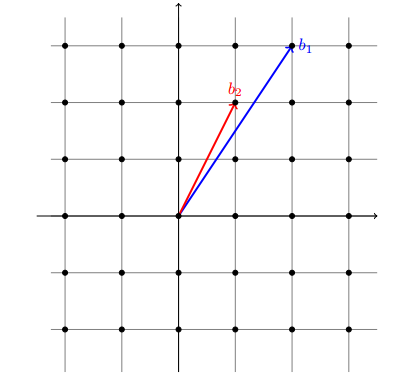
\includegraphics[scale=0.35]{lattices/2}
\centering
\caption{Lattice $\mathbb{Z}^2$ with a different basis consisting of vectors
$(1, 2)^t$ and $(2, 3)^t$}
\figuresubtitle{In fact, any lattice has infinitely many bases}
\end{figure}

    \item Below is a different lattice in $2$ dimensions, generated by the basis vectors $(2, 0)^t$ and $(1, 1)^t$. Note that this is a sub-lattice of $\mathbb{Z}^2$, namely a subset of $\mathbb{Z}^2$ which is also a lattice.
    

\begin{figure}[H]
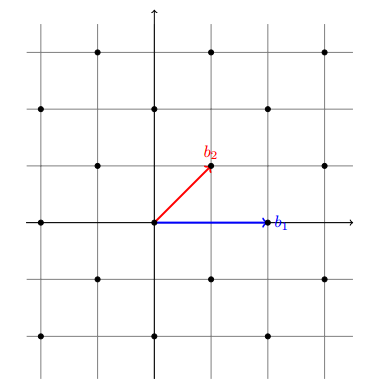
\includegraphics[scale=0.35]{lattices/3}
\centering
\caption{A full-rank lattice generated by the basis vectors $(1, 1)^t$ and $(2, 0)^t$}
\figuresubtitle{This is a sub-lattice of $\mathbb{Z}^2$}
\end{figure}   
    
    \item All the examples we saw so far are full-rank lattices. Below shows a lattice in $2$ dimensions generated by the vector $(1, 1)^t$, this lattice has a rank of $1$. The set of points generated by ${1}$ and ${\sqrt{2}}$ in one dimension is not a lattice. First, this example does not conform to definition of lattice, since ${1}$ and ${\sqrt{2}}$ are linearly dependent over $\mathbb{R}$. Secondly, any $n$-dimensional lattice is a discrete subset of $\mathbb{Z}^n$. However, the set generated by ${1}$ and ${\sqrt{2}}$ is not a discrete subset of $\mathbb{Z}$ since one can generate arbitrarily small numbers as linear combinations of ${1}$ and ${\sqrt{2}}$.

\begin{figure}[H]
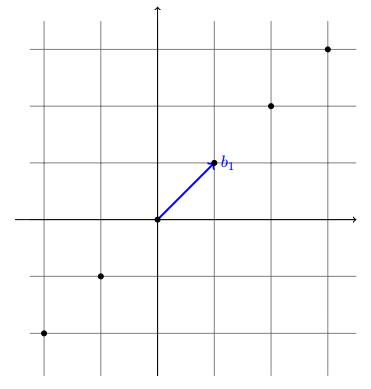
\includegraphics[scale=0.35]{lattices/4}
\centering
\caption{A non full-rank lattice with basis vector $(1, 1)^t$}
\figuresubtitle{Notice basis of lattice is not a square matrix (or full-rank)}
\end{figure}


\end{enumerate}










If a basis $\textbf{B}$ can be transformed by a multiplication with a transformation matrix $\textbf{U}$ such that the new basis $\textbf{B}'$ yields the same lattice as the original basis $\textbf{B}$ (i.e. $\textbf{B}' = \textbf{U} \times \textbf{B}, \mathcal{L}_\textbf{B} = \mathcal{L}_{\textbf{B}'})$, we refer to this transformation $\textbf{U}$ as a unimodular transformation. As such, any basis of a lattice can be transformed to any other basis for the same lattice through a multiplication with a single unimodular transformation matrix.


\subsection{Ideal lattices}
Research in lattice-based cryptography started with the publication of the public key encryption scheme by Ajtai and Dwork \cite{Ajtai:1997:PCW:258533.258604}, followed by schemes based on cyclic lattices, e.g. Micciancio introduced \cite{Mic07cyclic}. Later in \cite{Mic07cyclic} ideal lattices, a generalization of cyclic lattices, were introduced.

\textbf{Lattices via polynomial rings: }
Lattices cannot only be defined over $\mathbb{R}^n$ and $\mathbb{Z}^n$, but can also be defined via the ring $R = \mathbb{Z}_{q}[x]/ ( f(x) )$ where $R$ contains all polynomials in $x$ with integer coefficients modulo prime $q$ and polynomial $f(x)$. Note that if $f(x)$ is a monic polynomial, i.e. a polynomial with leading coefficient equal to $1$, then $R = \mathbb{Z}_{q}[x]/ ( f(x) )$ contains polynomials of degree at most $\text{deg}(f(x)) - 1$. We will focus on the case that $f(x)$ is a monic polynomial of degree $n$.

There is a map between elements from $R = \mathbb{Z}[x]/ ( f(x) )$, i.e. polynomials of bounded degree, and elements of a lattice $\mathcal{L}$, i.e. vectors, which is given as follows:

\begin{equation}
    \phi: a_1 + a_2x^1 + a_3x^2 + \dots + a_nx^{n-1} \mapsto (a_1, a_2, a_3 \dots , a_n)
\end{equation}



Here we will define ideal lattices and is based on Micciancio \cite{Mic07cyclic} and Lyubashevsky and Micciancio \cite{LyuMic06icalp}. First, recall that an ideal $I$, $I \subseteq R$ such that $I \neq \emptyset$, and for all $a, b \in I$ and $r \in R$, it holds that $-a \in I$, $a + b \in I$ and $ar \in I$.



A cyclic lattice is a lattice $\mathcal{L} \subseteq \mathbb{Z}^n$ with the property that if $(a_1, a_2, \dots , a_n) \in \mathcal{L}$ then also \\$(a_{i+1}, \dots , a_n, a_1, \dots , a_i) \in \mathcal{L}$ for all $i \in [1, n]$, \meaning that all rotations of a vector are contained in the lattice. Recall that vectors can also be expressed as polynomials, if $\mathcal{L}$ is a cyclic lattice isomorphic to $\mathbb{Z}[x] / ( x^n - 1 )$ and $\textbf{a}$ is a lattice vector, then also $x \textbf{a} \bmod x^n - 1$ is a lattice vector. This can be seen in following equation:

\begin{equation}
    x\textbf{a} = x \sum_{i=1}^n a_ix^{i-1} = \sum_{i=1}^n a_ix^i \equiv a_n + \sum_{i=1}^{n-1} a_ix^i \bmod x^n - 1
\end{equation}

Note that $x\textbf{a}$ corresponds to the cyclic shift $(a_n, a_1, \dots , a_{n-1})$. Inductively we have that also $x^i\textbf{a} \in \mathcal{L}$, for integer $i$. Only few lattices are cyclic lattices, thus needing a cyclic lattice is in practice very restrictive. Therefore the interest of researchers shifted to lattices isomorphic to $\mathbb{Z}[x]/( f(x) )$ for various monic $f(x)$, which has lead to a more general class of lattices, named \textit{ideal lattices}. To clarify, Ideal lattices are generalization of cyclic lattices.

\begin{definition}
\normalfont
Let $I$ be an ideal of $\mathbb{Z}[x]/(f(x))$ where $\text{deg}(f) = n$ and $\mathcal{L}_I = \{ (a_0, a_1, \dots, a_{n-1}) | a_0 + a_1x + \dots + a_{n-1}x^{n-1} \in I\}$. We call $\mathcal{L}_I$ an ideal lattice.
\end{definition}

This shows that the elements of an ideal lattice can be interpreted as polynomials from an ideal over $\mathbb{Z}[x]/( f(x) )$.


\begin{theorem}
\normalfont
Let $\mathcal{L}$ be a lattice that corresponds to an ideal in the ring $\mathbb{Z}[x]/( x^n + 1 )$ and let $\textbf{u} \in \mathcal{L}$ be a vector in lattice. Then the vectors: $\textbf{u}, x\textbf{u}, x^2\textbf{u}, \dots, x^{n-1}\textbf{u}$ are linearly independent.
\end{theorem}

Note that $x^n + 1$ is an irreducible polynomial when $n$ is a power of $2$. In case of cyclic lattices or lattices of the form $\mathbb{Z}[x] / ( x^n - 1 )$, is not ideal lattice because $x^n - 1$ is a reducible polynomial.


\subsection{Lattice problems}
The way lattices can be used in cryptography is by no means obvious, and was discovered in a breakthrough paper by Ajtai. His result has by now developed into a whole area of research whose main focus is on expanding the scope of lattice-based cryptography and on creating more practical lattice-based cryptosystems. Before discussing this area of research in more detail, let us first describe the the computational problems involving lattices, whose presumed hardness lies at the heart of lattice-based cryptography. Let $\mathcal{L}$ be a lattice of dimension $n$. The two fundamental computational problems in lattices are:

\begin{itemize}
    \item Shortest Vector Problem ($\mathrm{SVP}$): find a shortest non-zero vector in $\mathcal{L}$
    \item Closest Vector Problem ($\mathrm{CVP}$): given a vector $t \in \mathbb{R}^{n}$ not in $\mathcal{L}$, find a vector in $\mathcal{L}$ that is closest to $t$
\end{itemize}




\begin{definition}
\normalfont
Shortest Independent Vector Problem ($\mathrm{SIVP}$): given a basis of a lattice $\mathcal{L}$ and a parameter $q \in \mathbb{Z}$, find the shortest $q$ linearly independent lattice vectors (i.e. the set of lattice vectors $\textbf{b}_1, \dots, \textbf{b}_q$ contained within the minima $\lambda_q$)
\end{definition}


\begin{definition}
\normalfont
Closest Vector Problem ($\mathrm{CVP}$): let $\textbf{t}$ be some vector. The Closest Vector Problem is to find a vector $\textbf{v} \in \mathcal{L}$, such that $||\textbf{v} - \textbf{t}|| = \text{dist}(\textbf{t}, \mathcal{L})$ where $\text{dist}(\textbf{t}, \mathcal{L}) = \min_{\textbf{u} \in \mathcal{L}} ||\textbf{u} - \textbf{t}||$
\end{definition}


\begin{definition}
\normalfont
An instance of $\text{GapSVP}_{\gamma}$ (or decision $\text{SVP}_{\gamma}$) is given by an $n$-dimensional lattice $\mathcal{L}$ and a number $d > 0$. In YES instances, $\lambda_{1}(\mathcal{L}) \le d$ whereas in NO instances $\lambda_1(\mathcal{L}) > \gamma(n)\times d$
\end{definition}

The problem ${\text{GapSVP}_{\gamma}}$ consists of differentiating between the instances of $\text{SVP}$ in which the answer is at most $1$ or larger than $\gamma$, where $\gamma$ can be a fixed function of $n$, the number of vectors. Given a basis for the lattice, the algorithm must decide whether $\lambda(\mathcal{L})\leq 1$ or $\lambda (\mathcal{L})>\gamma$. Like other promise problems, the algorithm is allowed to error on all other cases.

\begin{definition}
\normalfont
An instance of $\text{SIVP}_{\gamma}$ is given by an $n$-dimensional lattice $\mathcal{L}$. The goal is to output a set of $n$-linearly independent lattice vectors of length at most $\gamma(n) \times \lambda_{n}(\mathcal{L})$
\end{definition}


\begin{definition}
\normalfont
Approximate Shortest Vector Problem ($\text{SVP}_{\gamma}$): given a lattice $\mathcal{L}$, the Approximate Shortest Vector Problem is to find a non-zero vector $\textbf{v} \in \mathcal{L}$, such that $||\textbf{v}|| \le \gamma \lambda_1 (\mathcal{L})$
\end{definition}


\begin{definition}
\normalfont
Approximate Closest Vector Problem ($\text{CVP}_{\gamma}$): let $\textbf{t}$ be some vector. The Approximate Closest Vector Problem is to find a vector $\textbf{v} \in \mathcal{L}$ such that $||\textbf{v} - \textbf{t}|| \le \gamma \text{ dist}(\textbf{t}, \mathcal{L})$ where $\text{dist}(\textbf{t}, \mathcal{L}) = \text{min}_{\textbf{u} \in \mathcal{L}} ||\textbf{u} - \textbf{t}||$
\end{definition}

Notice if $\gamma = 1$, then $\text{SVP}_{\gamma}$ and $\text{CVP}_{\gamma}$ would be the same as SVP and CVP

\begin{definition}
\normalfont
Bounded Distance Decoding Problem ($\text{BDD}_{\gamma}$): given $\mathcal{L}$ and a target point $\textbf{t} \in \mathbb{R}^{n}$ such that $\text{dist}(\textbf{t}, \mathcal{L}) \le \gamma \lambda_1(\mathcal{L})$, output a vector $\textbf{v} \in \mathcal{L}$ such that $||\textbf{v} - \textbf{t}|| \le \gamma \lambda_1(\mathcal{L})$
\end{definition}



In $\mathrm{SVP}$, a basis of a vector space $V$ and a $l_2$ norm are given for a lattice $\mathcal{L}$ and one must find the shortest non-zero vector in $V$, in $\mathcal{L}$. In other words, the algorithm should output a non-zero vector $\textbf{v}$ such that $||\textbf{v}||=\lambda (\mathcal{L})$. The closest vector problem is a generalization of the shortest vector problem. It is would be trivial to show that given an oracle for $\text{CVP}_{\gamma }$, one can solve $\text{SVP}_{\gamma }$ by making some queries to the oracle. However, the naive method to find the shortest vector by calling the $\text{CVP}_{\gamma }$ oracle to find the closest vector to $0$ does not work because $0$ is itself a lattice vector and the algorithm could potentially output $0$. The correct reduction is explained in \cite{Goldreich:1999:ASL:329343.329349}.

% \begin{theorem}
% \normalfont
% (Minkowski) For any lattice $\mathcal{L}$ and convex zero-symmetric set $S$ of volume $> 2^n \times \det(\mathcal{L})$, there exists a lattice point in $S$.
% \end{theorem}

\begin{theorem}
\normalfont
(Minkowski):
Let $\mathcal{L}$ be lattice of $\mathbb{R}^n$ with rank $n$, the length of shortest lattice vector of $\mathcal{L}$, $\lambda_1 \le \sqrt{n} \times \text{det}(\mathcal{L})^{\frac{1}{n}}$
\end{theorem}

The above theorem gives an upper bound of the length of shortest lattice vectors. Even though it is only a theorem of existence, the upper bound has significant practical interest. In the $\gamma$-approximation version $\text{SVP}_{\gamma}$, one must find a non-zero lattice vector of length at most $\gamma \lambda_1 (\mathcal{L})$ (note that vector $0$ is also in lattice). The exact version of the problem is only known to be NP-hard for randomized reductions \cite{Ajtai:1998:SVP:276698.276705} \cite{1366232}. Approach techniques: $\mathrm{LLL}$ lattice basis reduction algorithm which runs in polynomial time produces a relatively short vector in polynomial time, but does not solve the problem. HKZ basis reduction algorithm solves the problem in $\text{O}(n^{2n})$ time where $n$ is the dimension.

% By contrast, the equivalent problem with respect to the uniform norm is known to be NP-hard \cite{Khot:2005:HAS:1089023.1089027}.


\begin{figure}[H]
    \centering
    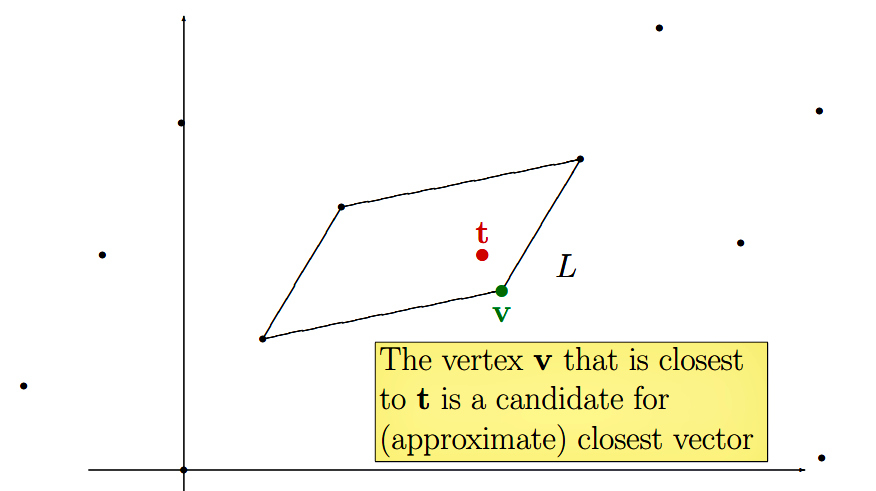
\includegraphics[width=6cm]{using-basis-to-solve-cvp}
    \caption{Visualization of $\mathrm{CVP}$ problem along with fundamental parallelepiped of lattice}
    \figuresubtitle{The vertex $v$ of the fundamental domain that is closest to $t$ will be a close lattice point if the basis is \textit{good}, meaning if the basis consists of short vectors that are reasonably orthogonal to one another.}
\end{figure}
    
    
    
\begin{figure}[H]
    \centering
    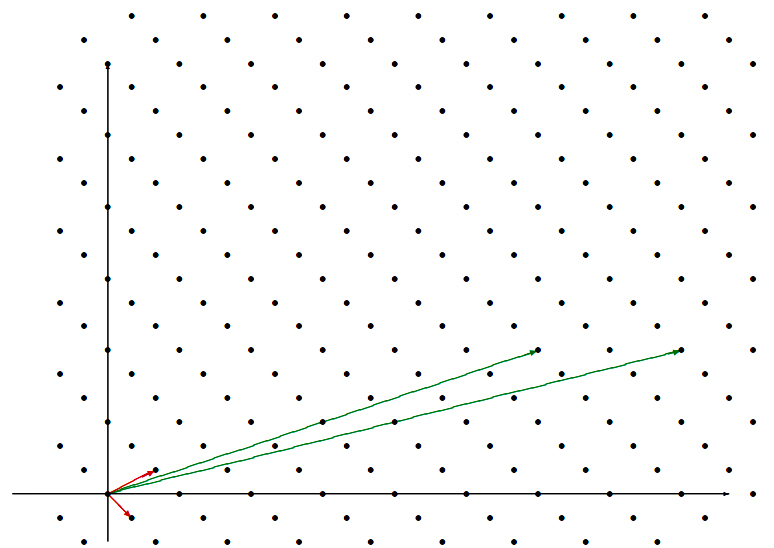
\includegraphics[width=6cm]{good-and-bad-basis}
    \caption{Visualization of two different lattice basis}
    \figuresubtitle{A \textit{good} basis that is short (in red) and a \textit{bad} basis that is relatively longer (in green)}
\end{figure}
    
    
    
\begin{figure}[H]
    \centering
    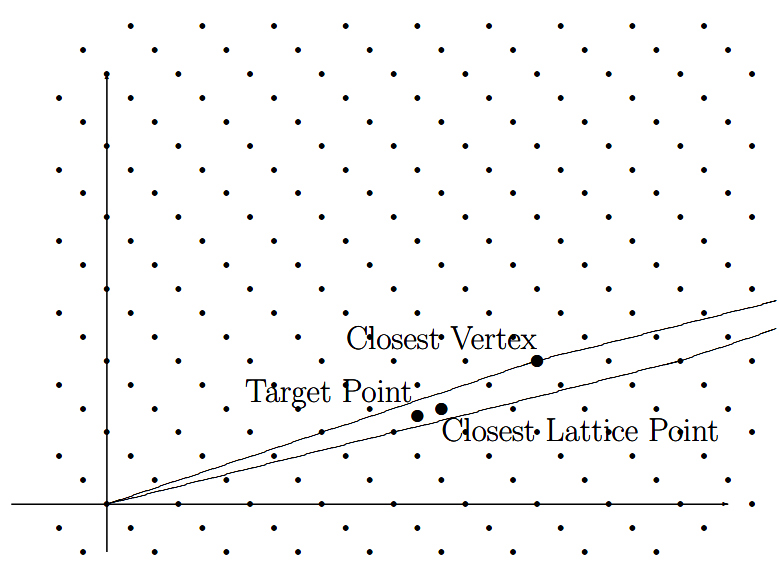
\includegraphics[width=6cm]{cvp-using-bad-basis}
    \caption{Visualization \textit{bad} lattice basis in solving $\mathrm{CVP}$ problem}
    \figuresubtitle{Here is the parallelogram spanned by a \textit{bad} basis and a $\mathrm{CVP}$ target point. It is easy to find the vertex of the parallelogram that is closest to the target point. However, the lattice point that actually solves $\mathrm{CVP}$ is much closer to the target than the closest vertex found using bad basis. Therefore, having an access to short lattice vectors would make CVP problem straightforward to solve. }
\end{figure}
    







\subsection{Worst-case hardness of lattice problems}
Let us describe Ajtai's result more precisely. The cryptographic construction given in \cite{ajtai1996generating} is known as a family of one-way functions. Ajtai proved that the security of this family can be based on the worst-case hardness of the $n^c$-approximate SVP for some constant $c$. In other words, the ability to invert a function chosen from this family with non-negligible probability implies an ability to solve any instance of $n^c$-approximate SVP. In his seminal papers, Ajtai showed that the SVP problem is NP-hard and discovered some connections between the worst-case complexity and average-case complexity of some lattice problems. Building on these results, Ajtai and Dwork created a public-key cryptosystem whose security could be proven using only the worst-case hardness of a certain version of SVP, thus making it the first attempt to use worst-case hardness to create secure systems \cite{Ajtai:1997:PCW:258533.258604}.

Strong security guarantees from worst-case hardness. Cryptography inherently requires average-case intractability, i.e., problems for which random instances drawn from a specified probability distribution are hard to solve. This is qualitatively different from the worst-case notion of hardness usually considered in the theory of algorithms and NP-completeness, where a problem is considered hard if there merely exist some intractable instances. Problems that appear hard in the worst-case often turn out to be easier on the average.

% especially for distributions that produce instances having some extra structure. For example, the existence of a secret key for decryption.

\begin{plain}
\normalfont
To solve $\mathrm{SIVP}$, an algorithm must work for any given input basis $\textbf{B}$. One can also formulate an average-case variant of $\mathrm{SIVP}$, where the input basis is generated at random according to some probability distribution.
\end{plain}










Ajtai in \cite{ajtai1996generating} gave connection between the worst-case and the average-case for lattices: he proved that certain problems are hard on the average (for cryptographically useful distributions), as long as some related lattice problems are hard in the worst-case. In details, Ajtai proved that, when $\textbf{A}$ in $f_\textbf{A}:\textbf{x} \mapsto \textbf{A}\textbf{x} \bmod q$ is chosen uniformly at random, a suitable restriction of function $f_\textbf{A}$ is at least as hard to invert on the average as the worst-case complexity of approximating certain lattice problems within a polynomial factor. Using results of this kind, one can design cryptographic constructions and prove that they are infeasible to break, unless all instances of certain lattice problems are easy to solve (worst implies any and average implies random). In essence, in lattice-based cryptosystem, for a fixed security parameter $n$, what the reduction shows is the existence of a solver for the lattice problem on input any $n$-dimensional lattice using the adversary breaking a lattice-based cryptosystem with the security parameter $n$ on the average-case. Therefore, since we can solve any instance, we can solve the hardest one of dimension $n$.

% We can convert any instance of the DL/CDH/DDH (discrete-log/computational DH/Decisional-DH) problem on the group to a random instance of the problem on the same group (this property is as known as the random self reducibility). Combining it with the previous reduction, we can say the security is based on the worst-case hardness of the problem over the \textit{fixed} group.



\begin{figure}[H]
    \centering
    
    \begin{figure}[H]
        \centering
        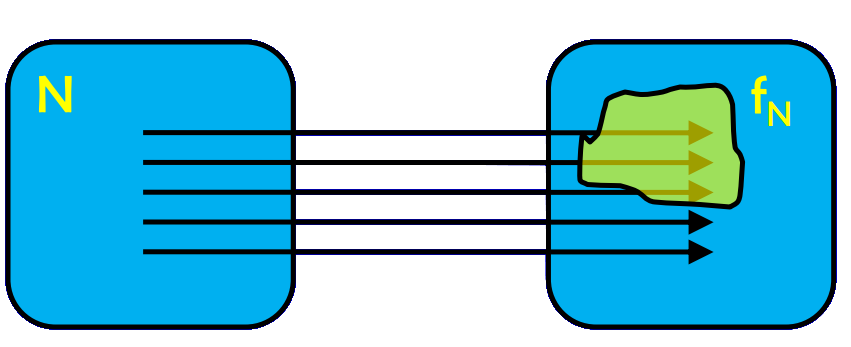
\includegraphics[width=5.2cm]{average-case}
        \caption{Average-case problem (e.g. factorization)}
    \end{figure}
    
    
    \begin{figure}[H]
        \centering
        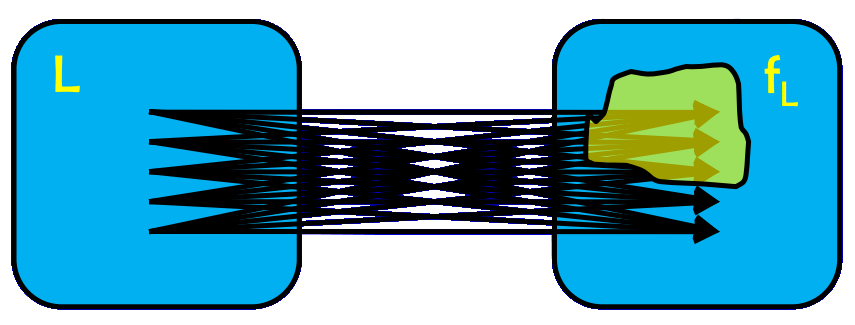
\includegraphics[width=5.2cm]{worst-case}
        \caption{Worst-case problem (e.g. lattice problems)}
    \end{figure}
    
    
    \caption*{
    \figuresubtitle{In average-case hardness, the cryptographic function is hard provided almost all $N$ are hard to factor; but in worst-case hardness the cryptographic function is hard provided the lattice problem is hard in the worst-case, this is a much stronger security guarantee and assures us that our distribution is correct. If we solve 1\% of lattice based cryptographic function, then we can solve \textit{all instances} of lattice problems.}
    }
\end{figure}

% Worst-case security guarantee is important because it assures us that attacks on the lattice based cryptographic construction are likely to be effective only for small choices of parameters and not asymptotically. In other words, it assures us that there are no fundamental flaws in the design of our cryptographic construction.

Following Ajtai’s worst-case to average-case reduction many different improvements on estimating SIS hardness have been done. This series of results is summed up in this theorem:

\begin{theorem}
\normalfont
(\cite{Micciancio:2007:WAR:1328722.1328733}, Theorem 5.16)
For any $m = poly(n)$, any $\beta > 0$, and any sufficiently large $q \ge \beta \cdot poly(n)$, solving SIS$_{n,q,\beta,m}$ is at least as hard as solving the decisional approximate shortest vector problem GapSVP$_{\gamma}$ and the approximate shortest
independent vectors problem SIVP$_\gamma$ on arbitrary $n$-dimensional lattices, for
some $\gamma = \beta \cdot poly(n)$.
\end{theorem}

The importance of the worst-case security guarantee is assurance  that there are no fundamental flaws in the design of our cryptographic construction.

\section{Lattice reduction}
The goal of lattice basis reduction is given an integer lattice basis as input, to find a basis with short, nearly orthogonal vectors. One measure of nearly orthogonal is the orthogonality defect. This compares the product of the lengths of the basis vectors with the volume of the parallelepiped they define. For perfectly orthogonal basis vectors, these quantities would be the same.

Any particular basis of $n$ vectors may be represented by a matrix $\textbf{B}$, whose columns are the basis vectors $\textbf{b}_{i}$, for $i=1, \dots, n$. In the fully dimensional case where the number of basis vectors is equal to the dimension of the space they occupy, this matrix is square, and the volume of the fundamental parallelepiped is simply the absolute value of the determinant of this matrix $\det(\textbf{B})$. If the number of vectors is less than the dimension of the underlying space, then volume is ${\sqrt {\det(\textbf{B}^{T}\textbf{B})}}$. For a given lattice $\mathcal{L}$, this volume is the same (up to sign) for any basis, and hence is referred to as the determinant of the lattice denoted by $\det(\mathcal{L})$ or lattice constant $d(\mathcal{L})$.

The orthogonality defect is the product of the basis vector lengths divided by the parallelepiped volume:
\begin{equation}
\delta (\textbf{B})= \frac{\Pi_{i=1}^{n}||\textbf{b}_{i}||}{\sqrt {\det(\textbf{B}^{T}\textbf{B})}} = \frac{\Pi _{i=1}^{n}||\textbf{b}_{i}||}{d(\mathcal{L} )}
\end{equation}

From the geometric definition it may be appreciated that $\delta (\textbf{B})\geq 1$ with equality if and only if the basis is orthogonal. If the lattice reduction problem is defined as finding the basis with the smallest possible defect, then the problem is NP-complete. However, there exist polynomial time algorithms to find a basis with defect $\delta (\textbf{B})\leq c \delta (\textbf{B})\leq c$ where $c$ is some constant depending only on dimension of the underlying space.

Although determining the shortest basis is an NP-complete problem, algorithms such as $\mathrm{LLL}$ algorithm can find a short, \textit{not necessarily shortest}, basis in polynomial time with guaranteed worst-case performance. The following example demonstrates the computation of lattice reduction algorithm by which we can reduce original basic matrix from: $\textbf{B} = \begin{psmallmatrix}     1 & 2 \\     3 & 4 \\ \end{psmallmatrix} \to \textbf{B}' = \begin{psmallmatrix}    1 & 0 \\    0 & 2 \\ \end{psmallmatrix}
$ and matrix of $\textbf{U} = \begin{psmallmatrix}    -2 & 1 \\    3 & -1 \\ \end{psmallmatrix}
$ is a unimodular matrix with determinant of $\text{-1}$. Also, $\mathcal{L}(\textbf{B}) = \mathcal{L}(\textbf{B}')$ because: $\textbf{B}' = \textbf{B} \times \textbf{U}$. 
\begin{figure}[H]
\centering
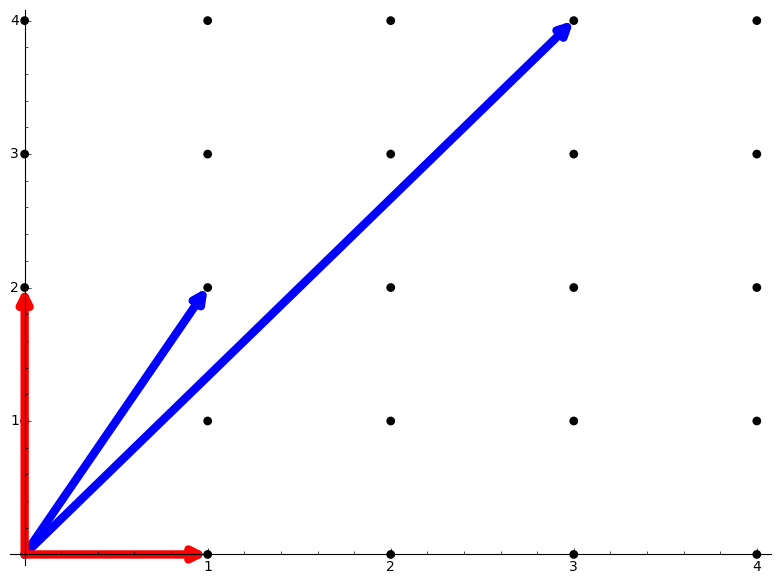
\includegraphics[width=4.5cm]{basic_lattice}
\caption{Lattice generated by vectors: $\textbf{v}_1 = (1, 2)$ and $\textbf{v}_2 = (3, 4)$}
\figuresubtitle{Reduced basis consisting of vectors: $\textbf{v}'_1 = (1,0)$ and $\textbf{v}'_2 = (0,2)$ generates the same lattice}
\end{figure}









\subsection{\texorpdfstring{$\mathrm{LLL}$}{LLL} algorithm}
The Lenstra–Lenstra–Lovász ($\mathrm{LLL}$) lattice basis reduction algorithm is a polynomial time lattice reduction algorithm invented by A. Lenstra, H. Lenstra and L. Lovász in 1982 \cite{Lenstra1982}. Given a basis ${\mathbf {B}}=\{{\mathbf  {b}}_{1},{\mathbf{b}}_{2},\dots ,{\mathbf{b}}_{d}\}$ with $n$-dimensional integer coordinates, for a lattice $\mathcal{L}$ with $d\leq n$, $\mathrm{LLL}$ algorithm calculates an $\mathrm{LLL}$-reduced (short, nearly orthogonal) lattice basis in time $\text{O}(d^{5}n\log ^{3}B)$, where $B$ is the largest length of $\textbf{b}_{i}$ under the Euclidean norm and $d$ is referring to number of basis vectors in $\textbf{B}$ (we should use $d$ because the dimension of the lattice might be smaller than the dimension of the $\mathbb{R}^n$ that the lattice is embedded in). 

% The original applications were to give polynomial-time algorithms for factorizing polynomials with rational coefficients, for finding simultaneous rational approximations to real numbers, and for solving the integer linear programming problem in fixed dimensions.

$\mathrm{LLL}$ can be used as a cryptanalysis tool (i.e., to break cryptography):

\begin{enumerate}
    \item Knapsack-based cryptosystem \cite{doi:10.1137/0215038} (appendix A describes in details how $\mathrm{LLL}$ breaks early knapsack cryptosystem)
    \item RSA when the public exponent $e$ is small or when partial knowledge of the secret key is available \cite{Wang:2015:MFP:2901632} \cite{Coppersmith:2001:FSS:648244.753513}. $\mathrm{LLL}$ is used to find a polynomial that has the same zeroes as the target polynomial but smaller coefficients. 
\end{enumerate}



% \subsection{Gram-Schmidt Orthogonalization}
In order to achieve an orthogonal basis, an iterative process can be taken whereby each vector is projected onto a hyperplane perpendicular to the previous vectors. The Gram-Schmidt Orthogonalization algorithm is an iterative approach to orthogonalizing the vectors of a basis. The first vector $\textbf{b}_1$ of a given basis $\textbf{B}$ is taken as a reference and the second vector $\textbf{b}_2$ is projected on to an $(n - 1)$-hyperplane perpendicular to $\textbf{b}_1$. The third vector $\textbf{b}_3$ is projected onto a $(n - 2)$-hyperplane perpendicular to the plane described by $\textbf{b}_1$ and $\textbf{b}_2$. This process continues in an iterative fashion until all degrees of freedom are exhausted. The new orthogonal vectors are denoted $\textbf{b}^*_i$ and the new basis as $\textbf{B}^*$.


\begin{equation}
\begin{split}
	\textbf{b}^{*}_{i} = \textbf{b}_i - \sum_{j=1}^{i-1}{\mu_{i, j}\textbf{b}^*_j}\\
	\mu_{i, j} = \frac{\langle \textbf{b}_i , \textbf{b}_j^*\rangle}{\langle \textbf{b}_j^*, \textbf{b}_j^*\rangle}
\end{split}
\end{equation}

% It should be noted that $\{ \textbf{b}_1^{*}, \textbf{b}_2^{*}, \dots, \textbf{b}_n^{*} \}$ is usually not a basis of $\mathcal{L}$ as vectors may not be in lattice. Also, determinant of $\mathcal{L}$ satisfies:

% \[  \text{det}(\mathcal{L}) = \prod_{ 1 \le i \le n} ||\textbf{b}_i^{*}||, \text{det}(\mathcal{L}) \le \prod_{1 \le i \le n} ||\textbf{b}_i||\]


\begin{figure}[H]
\centering
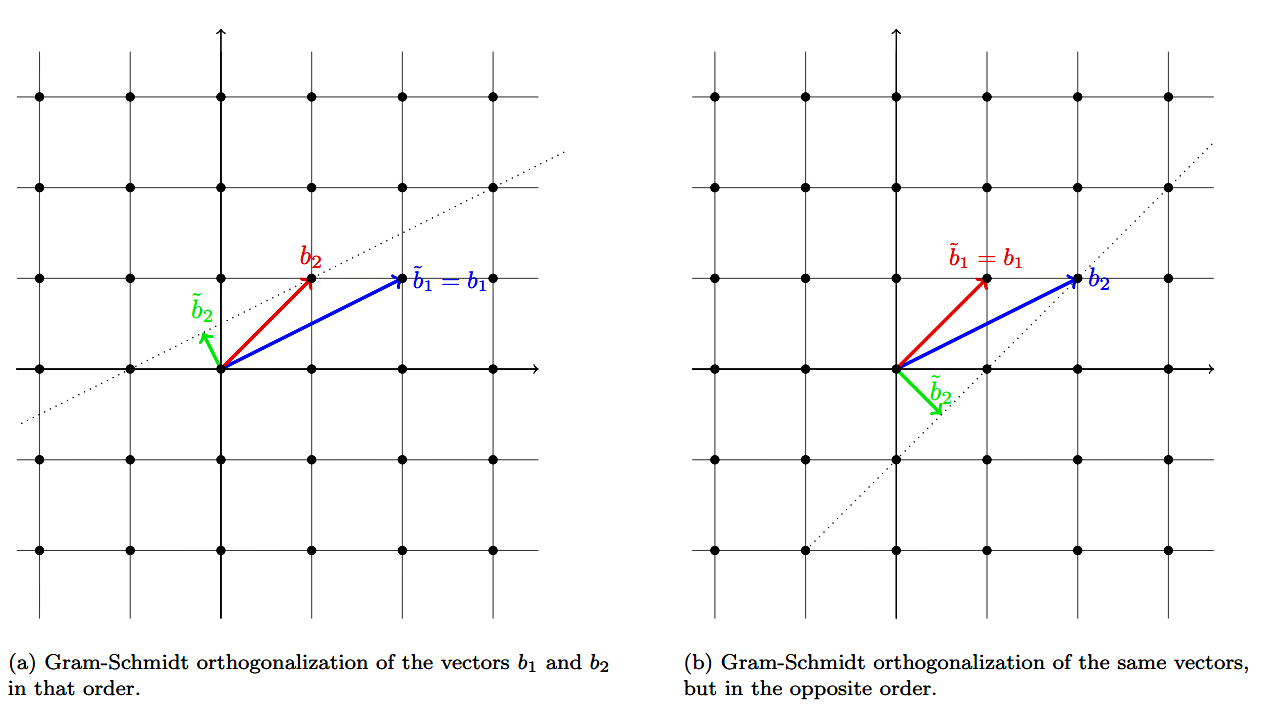
\includegraphics[scale=0.3]{gram-schmidt-not-in-lattice}
\caption{Gram-Schmidt Orthogonalization.}
\figuresubtitle{The vectors $\textbf{b}_{1}^{*}, \dots, \textbf{b}_{n}^{*}$ do not form a lattice basis. In fact, the Gram-Schmidt vectors are not necessarily in the lattice.}
\end{figure}



% \subsection{\texorpdfstring{$\mathrm{LLL}$}{LLL} reduction}
The precise definition of $\mathrm{LLL}$-reduced basis is as follows: Given a basis ${\textbf{B}}=\{{\mathbf{b}}_{0},{\mathbf{b}}_{1},\dots ,{\mathbf{b}}_{n}\}$,
define its Gram–Schmidt process orthogonal basis: ${\mathbf{B}}^{*}=\{{\mathbf{b}}_{0}^{*},{\mathbf  {b}}_{1}^{*},\dots ,{\mathbf  {b}}_{n}^{*}\}$, and the Gram-Schmidt coefficients
$\mu _{{i,j}}={\frac  {\langle {\textbf  {b}}_{i},{\textbf  {b}}_{j}^{*}\rangle }{\langle {\textbf{b}}_{j}^{*},{\textbf  {b}}_{j}^{*}\rangle }}$, for any $1\leq j<i\leq n$.

Then the basis $\textbf{B}$ is $\mathrm{LLL}$-reduced if there exists a parameter $\delta  \in (0.25,1]$ such that the following holds:

\begin{enumerate}
    \item (size-reduced) For $1\leq j<i\leq n\colon \left|\mu _{{i,j}}\right|\leq 0.5$. By definition, this property guarantees the length reduction of the ordered basis.
    \item (Lovász condition) For $k = 1,2, \dots,n \colon \delta \Vert {\mathbf  {b}}_{{k-1}}^{*}\Vert ^{2}\leq \Vert {\mathbf  {b}}_{k}^{*}\Vert ^{2}+\mu _{{k,k-1}}^{2}\Vert {\mathbf  {b}}_{{k-1}}^{*}\Vert ^{2}$. Here, estimating the value of the $\delta$  parameter, we can conclude how well the basis is reduced. Greater values of $\delta$ lead to stronger reductions of the basis.    
\end{enumerate}







\begin{plain}
\normalfont
The first condition assures the resulting basis is nearly orthogonal. But length reduction alone does not guarantee near orthogonality.
\end{plain}

The issue with the length-reduction criterion alone (and the reason the Lovász condition is included in the $\mathrm{LLL}$ algorithm) is that the following basis satisfies it:

\begin{figure}[H]
\centering
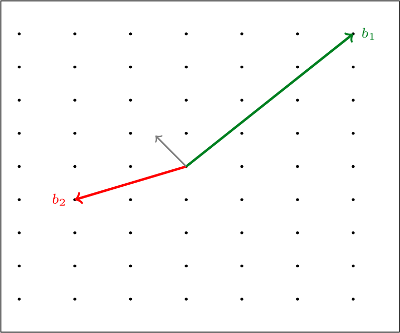
\includegraphics[width=5cm]{bad-reduction}
\caption{Length-reduced lattice basis}
\figuresubtitle{The grey arrow is the projection of $\textbf{b}_2$ to the orthogonal complement of $\textbf{b}_1$}
\end{figure}

Clearly, this basis is not very short, nor is it close to being orthogonal (i.e., note that length reduction alone does not necessary imply almost-orthogonality). The Lovász condition is suited to detect such a situation: If the order of the vectors is swapped, another length reduction can easily be performed, yielding the following $\mathrm{LLL}$-reduced basis:

\begin{figure}[H]
\centering
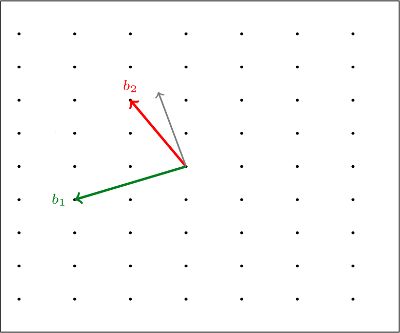
\includegraphics[width=5cm]{good-reduction}
\caption{$\mathrm{LLL}$-reduced lattice basis}
\end{figure}

A. Lenstra, H. Lenstra and L. Lovász have noticed that a situation in which length reduction alone is stuck with a very bad basis - as depicted in the first image - always has vectors which are in the \quotes{wrong} order comparing their lengths and which are far from being orthogonal, and that it helps in this case to exchange them and continue length-reducing. That is really the core idea of the $\mathrm{LLL}$ algorithm.

% \[(\delta-\mu_{i+1,i})\lVert \textbf{b}_i^\ast\rVert^2 \;\leq\; \lVert \textbf{b}_{i+1}^\ast\rVert^2\]

% The Gram-Schmidt coefficient $\mu_{i+1,i}$ measures the angle between $\textbf{b}_i^\ast$ and $\textbf{b}_{i+1}$; the angle is small if and only if $\mu$ is close to $1$, and it is large (i.e. almost orthogonal) if and only if $\mu$ is close to $0$. Note this talks about the angle between the orthogonalized vector $\textbf{b}_i^\ast$ and the lattice vector $\textbf{b}_{i+1}$, but $\textbf{b}_i^\ast$ is in turn forced to be quite close to $\textbf{b}_i$, hence this also bounds the angle between the lattice basis vectors depending on the orthogonalized vectors' lengths relative to each other.

In summary, the Lovász condition is fulfilled if the vectors are close enough to being orthogonal, or if they are roughly ordered by length. Both of these properties lead to length reduction being quite effective. Initially, A. Lenstra, H. Lenstra and L. Lovász demonstrated the $\mathrm{LLL}$-reduction algorithm for $\delta ={\frac{3}{4}}$. Note that although $\mathrm{LLL}$-reduction is well-defined for $\delta =1$, the polynomial-time complexity is guaranteed only for $\delta \in (0.25,1)$.

% The $\mathrm{LLL}$ algorithm computes $\mathrm{LLL}$-reduced bases. There is no known efficient algorithm to compute a basis in which the basis vectors are as short as possible for lattices of dimensions greater than 4. However, an $\mathrm{LLL}$-reduced basis is nearly as short as possible, in the sense that there are absolute bounds $c_{i}>1$ such that the first basis vector is no more than $c_{1}$ times as long as a shortest vector in the lattice, the second basis vector is likewise within $c_{2}$ of the second successive minimum, and so on.



The following description of $\mathrm{LLL}$ algorithm is based on (Hoffstein, Pipher \& Silverman 2008 \cite{Hoffstein:2008:IMC:1481183}, Theorem 6.68), \textbf{Input:}

\begin{enumerate}
    \item a lattice basis $\textbf{b}_{0}, \textbf{b}_{1},\dots ,\textbf{b}_{n}\in \mathbb{Z}^{m}$
    \item parameter $\delta$  with ${\frac{1}{4}}<\delta <1$, most commonly $\delta ={\frac{3}{4}}$ 
\end{enumerate}

\begin{algorithm}[H]
    \begin{algorithmic}
        \caption{$\mathrm{LLL}$ lattice reduction Algorithm}
        \label{LLL}
        \Procedure{LLL}{$\textbf{b}, \delta$}\Comment{Basis and delta}
        \State $ortho:=\mathrm{gramSchmidt} (\{\textbf{b}_{0}, \dots, \textbf{b}_{n}\})=\{\textbf{b}_{0}^{*}, \dots, \textbf{b}_{n}^{*}\}$
        \item[] 
        \Comment{$\textbf{b}\gets $ Perform Gram-Schmidt, but do not normalize}
        \State Define $\mu_{i,j}:= \frac{\langle \textbf{b}_{i},\textbf{b}_{j}^{*}\rangle}{\langle \textbf{b}_{j}^{*}, \textbf{b}_{j}^{*}\rangle}$, which must always use the most current values of $\textbf{b}_{i}, \textbf{b}_{j}^{*}$.
        \State $k \gets 1$
        \While{$k\leq n$}
            \For{$j \textbf{ form } k-1 \textbf{ to } 0$}
                \If{$|\mu_{k,j}|>\frac{1}{2}$}
                {$\textbf{b}_{k}=\textbf{b}_{k}-\lfloor \mu_{k,j}\rceil \textbf{b}_{j}$}
                \item[] \Comment{Update ortho entries and related $\mu _{i,j}$'s as needed}
                \item[] \Comment{Naive method is to recompute $ortho:=\mathrm{gramSchmidt} (\{\textbf{b}_{0}, \dots, \textbf{b}_{n}\})=\{\textbf{b}_{0}^{*}, \dots, \textbf{b}_{n}^{*}\}$ when a $\textbf{b}_{i}$ changes)}
                \EndIf
            \EndFor
            \If{$\langle \textbf{b}_{k}^{*}, \textbf{b}_{k}^{*}\rangle \geq (\delta -(\mu _{{k,k-1}})^{2})\langle \textbf{b}_{{k-1}}^{*}, \textbf{b}_{{k-1}}^{*}\rangle$}
            \State {$k=k+1$}
            \Else{}
                \State {$\textbf{swap } \textbf{b}_{k} \textbf{ and } \textbf{b}_{k-1}$}
                \Comment{Update ortho entries and related $\mu _{i,j}$'s as needed}
                \State $k=\max(k-1,1)$
            \EndIf
        \EndWhile
            \item[] 
            \State \textbf{return:} $\mathrm{LLL}$ reduced basis $\textbf{b}_{0}, \textbf{b}_{1}, \dots, \textbf{b}_{n}$
        \EndProcedure
    \end{algorithmic}
\end{algorithm}


\subsection{The BKZ reduction algorithm}
Blockwise Korkine-Zolotarev (or $\mathrm{BKZ}$) reduction is a reduction algorithm for lattices. It has been introduced by Schnorr and Euchner \cite{Schnorr93latticebasis}. The $\mathrm{BKZ}$ algorithm uses so called local blocks to achieve reduction, hence the name. The quality of the reduction that is achieved by $\mathrm{BKZ}$ reduction depends on this block size. Increasing block sizes also mean an improvement in the reduction. The $\mathrm{BKZ}$ algorithm starts by $\mathrm{LLL}$-reducing a given basis of a lattice. The quality of the reduction is then iteratively improved. This improvement is achieved using the local blocks determined by the input basis and the block size.


Running $\mathrm{BKZ}$ algorithm with large block size results in shorter and more orthogonal basis in compassion with $\mathrm{LLL}$, hence it can be used to attack underlying lattice of $\mathrm{LWE}$.

% The size of most of these blocks is determined by an additional input parameter for the algorithm,
% called the block size $\beta$.

% The first block consists of the first basis vector and the $\beta - 1$ succeeding ones. The second block is constructed similarly but introduces a slight modification: Instead of taking the second basis vector and $\beta$ succeeding ones, their projections onto the orthogonal complement of the first basis vector are used. The remaining blocks are constructed in the same way: For block $i$, the basis vectors with index $j$, satisfying $i \ge j < i + \beta$, are projected onto the orthogonal complement of the vector space spanned by all basis vectors $\textbf{b}_m$, where $m < i$. This projection forms the so called local block. The index $l$ of the last vector in a block is computed as $l = \text{min}(i + \beta - 1, n)$, where $n$ is the dimension of the lattice. That means that the block starting at index $n - \beta + 1$ is the last one of size $\beta$. From there on, the size of the last blocks decreases step by step. The local blocks are also called local projected blocks because of the way they are constructed.
% The actual improvement is achieved as follows: Each of the local blocks defines a lattice. Each iteration looks at one block and ensures that the first vector of the block is the shortest vector inside the lattice spanned by this block. If this is not already the case, the shortest vector of the lattice is inserted into the block. The inserted vector is inside the lattice, and therefore linear dependent on the basis vectors. This means that after inserting the new vector, the local block is not a basis for the local lattice any longer. To obtain a basis again, the $\mathrm{LLL}$ algorithm is called on the expanded block. Note that the procedure call of the $\mathrm{LLL}$ algorithm is executed for each local block, no matter whether an insertion took place or not.

% The block size determines the dimension of most of the local projected lattices in which shortest vectors have to be found. It also determines the amount of basis vectors that are used as input for the $\mathrm{LLL}$ algorithm after insertion of a new vector into the local block.

% Running $\mathrm{BKZ}$ algorithm with large block size results in shorter and more orthogonal basis in compassion with $\mathrm{LLL}$, hence can be used to attack underlying lattice of $\mathrm{LWE}$.




\section{Short integer solution problem (\texorpdfstring{$\mathrm{SIS}$}{SIS})}
% (and it Ring variant, Ring-$\mathrm{SIS}$)
$\mathrm{SIS}$ is an average case problem that is used in lattice-based cryptography constructions. Lattice-based cryptography began in 1996 from a seminal work by Ajtai who presented a family of one-way functions based on SIS problem. He showed that it is secure in average-case if $\mathrm{SVP}_{\gamma }$ (where $\gamma =n^{c}$ for some constant $c > 0$) is hard in worse-case scenario.



A trapdoor function is a function that is easy to perform one way, but has a secret that is required to perform the inverse calculation efficiently. That is, if $f$ is a trapdoor function, then $y=f(x)$ is easy to compute, but $x=f^{-1}(y)$ is hard to compute without some special knowledge $k$. Given $k$, then it is easy to compute $y=f^{-1}(x,k)$. The analogy to a \quotes{trapdoor} is something like this: It is easy to fall through a trapdoor, but it is very hard to climb back out and get to where we started unless we have a ladder.

Hash-function is not a trapdoor function because it is not reversible. Instead, it is called a one-way function. One-way function is similar to a trapdoor function in that it's easy to compute and it's very hard to reverse, but there is no special key that allows to reverse the one-way function. For example: RSA is a trapdoor function because it's inverse which is a factorization is hard, but SHA-3 is just a one-way hash function as it's output can be hash of more that one inputs since hash functions are not a one-to-one function.

\begin{definition}
\normalfont
Given parameters $m,n,q \in \mathbb{Z}$, key $\textbf{A} \in \mathbb{Z}^{n\times m}_{q}$ and input $\textbf{x} \in \{0,1\}^m$, Ajtai's one-way hash function is a function that outputs $f_{\textbf{A}}(\textbf{x}) = \textbf{A}\textbf{x} \bmod q$
\end{definition}



\begin{figure}[H]
    \centering
    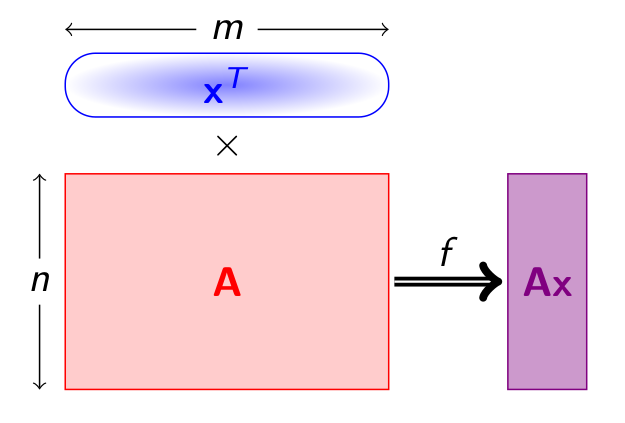
\includegraphics[scale=0.2]{ajtai}
    \caption{Visualization of Ajtai's one-way function}
\end{figure}




\iftoggle{verylong}{
\lstinputlisting[language=Python, caption=Ajtai hash function given a secret matrix \textit{m} random value \textit{x} which is a column vector]{code_snippets/ajtai_hash_function.sage}
}{}

% \begin{plain}
% \normalfont
% Note that modular class of lattices are lattices for which asymptotic worst-case to average-case connections holds. For more details refer to \cite{ajtai1996generating}.
% \end{plain}

\begin{theorem}
\normalfont
For $m > n \log q$, if lattice problems (i.e. $\mathrm{SIVP}$) are hard to approximate in the
worst-case, then $f_{\textbf{A}}(\textbf{x}) = \textbf{A}\textbf{x} \bmod q$ is a one-way function.
\end{theorem}






\begin{definition}
\normalfont
$\text{SIS}_{n,m,q,\beta}$: let $\textbf{A}\in \mathbb{Z}_{q}^{n\times m}$ be an $n\times m$ matrix with entries in $\mathbb{Z} _{q}$ that consists of $m$ uniformly random vectors $\textbf{a}_{i}\in \mathbb{Z}_{q}^{n}: \textbf{A}=( \textbf{a}_{1},\cdots ,\textbf{a}_{m})$. Find a nonzero vector $\textbf{x}\in \mathbb{Z}^{m}$ such that:

\begin{itemize}
    \item $\|\textbf{x}\|\leq \beta $
    \item $f_{\textbf{A}}(\textbf{x}):\textbf{A}\textbf{x}=0\in \mathbb {Z}_{q}^{n}$
\end{itemize}
\end{definition}


\begin{figure}[H]
    \centering
    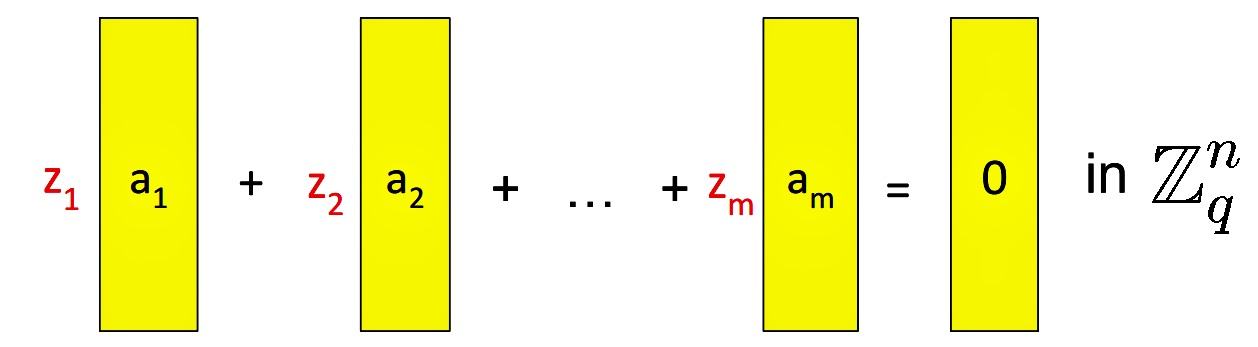
\includegraphics[scale=0.2]{SIS}
    \caption{Visualization of $\mathrm{SIS}$ problem introduces by Ajtai}
\end{figure}

It should be noted that a solution to $\mathrm{SIS}$ without the required constrain on the length of the solution is easy to compute by using Gaussian elimination technique. We also require $\beta <q$, otherwise $x=(q,0,\ldots ,0)\in \mathbb{Z}^{m}$ is a trivial solution.



In order to guarantee $f_{\textbf{A}}(\textbf{x})$ has non-trivial, short solution, we require:
\begin{itemize}
    \item $\beta \geq \sqrt{n\log q}$, and
    \item $m\geq n\log q$ (to get compression)
\end{itemize}


% \begin{theorem}
% \normalfont
% For any $m=\operatorname {poly} (n)$, any $\beta >0$, and any sufficiently large $q\geq \beta n^{c}$ (for any constant $c > 0$), solving $\mathrm{SIS}_{n,m,q,\beta }$ with non-negligible probability is at least as hard as solving the $\mathrm{GapSVP}_{\gamma }$ and $\mathrm{SIVP}_{\gamma}$ for some $\gamma =\beta \times \mathcal{O}(\sqrt {n})$ with a high probability in the worst-case scenario.

% \end{theorem}

\begin{plain}
\normalfont
$\mathrm{SIS}$ problem can also form a collision-Resistant Hash function:

Given: $\textbf{A}=(\textbf{a}_1,\dots,\textbf{a}_m) \in \mathbb{Z}^{n\times m}_{q}$, define $\mathrm{Hash}_{\textbf{A}}: \{0,1\}^{m} \mapsto \mathbb{Z}^{n}_{q}$ where $\mathrm{Hash}_{\textbf{A}}(z_1, \dots,z_m) = a_1 z_1 + \dots + a_m z_m$. Domain of $h = \{0,1\}^{m}$ (size $= 2^m$). Range of $h = \mathbb{Z}^{n}_{q}$ (size $= q^n$). Set $m > n\log q$ to get compression. Collision would occur when:

\begin{equation}
\textbf{a}_1z_1 + \dots + \textbf{a}_mz_m = \textbf{a}_1y_1 + \dots + \textbf{a}_my_m
\end{equation}

By adjusting the above we get: $\textbf{a}_1(z_1-y_1) + \dots + \textbf{a}_m(z_m-y_m) = 0$ and $z_i-y_i$ are in $\{-1,0,1\}$. Nothing happens as trivial solution is not a valid solution to $\mathrm{SIS}$ problem, further because the only way we could find a collision is when $z_i-y_i = 0 \bmod q$. So $\mathrm{SIS}$ is a collision resistant hash function.  
\end{plain}

Regrading the efficiency of Ajtai's trapdoor function, matrix multiplication of $1 \times m$ matrix with $m \times n$ matrix would yield $\text{O}( m n)$ time complexity. Hence, it is efficient in run-time but has very high space needs. The space needs can be reduced by number of ways. One idea could be use a structured matrix i.e. take the first row and the second row would be one bit left/ right circular of the first row and so on allowing just the first row of the matrix to be stored as the public key. Hermite Normal form (i.e. upper triangular matrix) could also be used for the public key to reduce half of the size of the matrix.


In 1996, Ajtai showed that, for good parameters, if there exists an inverter of his hash functions, then there exists an algorithm finding a short vector from any $n$-dimensional lattice. Goldreich, Goldwasser, and Halevi pointed out if there exists an algorithm that finds a collision in the Ajtai hash function, then there exist an algorithm that finds a short vector from any $n$-dimensional lattice. The reductions are based on the fact that the sum of short vectors is (relatively) short.

\subsection{Interpreting \texorpdfstring{$\mathrm{SIS}$}{SIS} problem in lattice words and lattice reduction}
Define a lattice related to a matrix $\textbf{A}\in \mathbb{R}^{n \times m}$ as

\[\Lambda = \Lambda_q^{\perp}({\textbf{A}}) = \{\textbf{e} \in \mathbb{Z}^m \mid {\textbf{A}} \textbf{e} \equiv \textbf{0} \bmod{q}\}\]

This $\Lambda$ is an $m$-dimensional $q$-ary lattice that corresponds to the linear code with parity check matrix equal to $\textbf{A} \bmod q$ (we can check this is a lattice by verifying that for any two vectors $\textbf{e}, \textbf{e}' \in \Lambda$, the sum of them lies in $\Lambda$ again. We can check this is $m$-dimensional by verifying that any $q \textbf{u}_i$ is in $\Lambda$, where $\textbf{u}_i$ is a unit vector).

This lattice defines a map from $\mathbb{Z}^m$ to a quotient group $\mathbb{Z}^m/\Lambda$. The map is a hash function. Conversely, a collision $\textbf{e} \neq \textbf{e}'$ for $f_{\textbf{A}}$ implies a short non-zero vector $\textbf{e}-\textbf{e}'$ in $\Lambda_q^{\perp}({\textbf{A}})$.


Solving $\mathrm{SIS}$ (or breaking Ajtai's trapdoor function) comes down to finding a short vector in the underlying lattice (or $\Lambda_q^{\perp}$). Lattice basis reduction methods like $\mathrm{LLL}$ help in the sense that they can reduce a basis with long lattice vectors to a basis with shorter, more orthogonal lattice vectors. If the reduction is strong enough (e.g. $\mathrm{BKZ}$ with large enough block size) then we can expect that the first basis vector of the reduced basis is a solution to $\mathrm{SIS}$ (how strong the basis reduction should be to find a solution depends on $n, m, q$). To summarize, $\mathrm{LLL}$ can solve the easiest $\mathrm{SIS}$ instances, and can assist in solving harder $\mathrm{SIS}$ instances by finding a shorter basis, which makes finding even shorter lattice vectors a bit easier.


Finding a short nonzero $z \in \Lambda_q^{\perp}(\textbf{A})$ for uniformly random $\textbf{A} \in \mathbb{Z}_q^{n \times m}$, where $m \approx n \log q$ ($\mathrm{SIS}$ problem) can be reduced to solving $\mathrm{GapSVP}_{\beta\sqrt{n}}$, $\mathrm{SIVP}_{\beta\sqrt{n}}$ on any $n$-dimensional lattice. In essence, let $\textbf{S}$ be the set of all integer $z = (z_1, \dots z_n)$ such that $z_1\times{\textbf{a}_{1}}, \dots, z_n\times{\textbf{a}_{n}} = 0 \bmod q$, then $\textbf{S}$ is a lattice and $\mathrm{SIS}$ problem asks to find a short vector in $\textbf{S}$. $\mathrm{SIS}$ problem is a an average-case hard problem but $\mathrm{SVP}$ problem is a worst-case hard problem.


\begin{figure}[H]
\centering
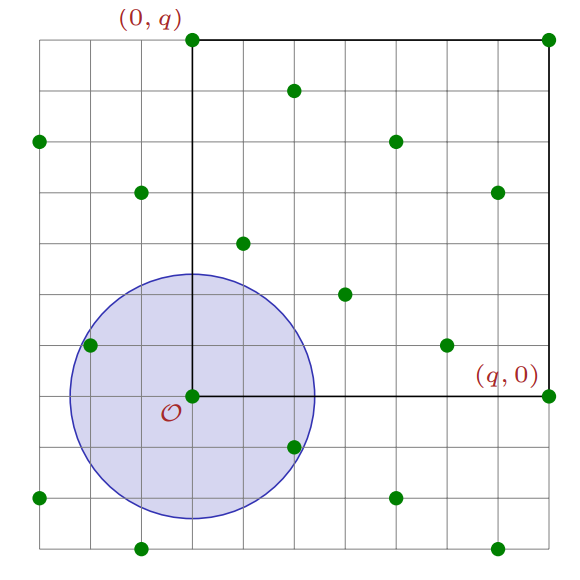
\includegraphics[width=4.5cm]{sis-to-svp}
\caption{Visualization of $\mathrm{SIS}$ reduced to $\mathrm{GapSVP}_{\beta\sqrt{n}}$, $\mathrm{SIVP}_{\beta\sqrt{n}}$}
\figuresubtitle{Notice that we are looking for smallest radius to contain enough lattice points to reconstruct the lattice itself.}
\end{figure}





\section{\texorpdfstring{$\mathrm{LWE}$}{LWE} and lattice cryptography}
The learning with errors ($\mathrm{LWE}$) problem is to efficiently distinguish between vectors created from a \quotes{noisy} set of linear equations versus uniformly random vectors. Given a matrix $\textbf{A} \in \mathbb{Z}^{m \times n}_q$ and a vector $\textbf{v} \in \mathbb{Z}^m_q$, the goal is to determine whether $\textbf{v}$ has been sampled uniformly at random from $\mathbb{Z}^m_q$ or whether $\textbf{v} = \textbf{A}\textbf{s} + \textbf{e}$ for some random $\textbf{s} \in \mathbb{Z}^m_q$ and $\textbf{e} \in \chi_m$, where $\chi$ is a small \quotes{noise} distribution over $\mathbb{Z}_q$.

$\mathrm{LWE}$ problem is very closely related to coding theory. If we choose the parameter $q = 2$, this becomes the well-studied learning parity with noise ($\mathrm{LPN}$) problem, which is believed to be hard. Recovering the key from the more general $\mathrm{LWE}$ problem is essentially equivalent to decoding a noisy linear code, also a long established difficult problem in coding theory. However, for modern cryptographic purposes it is more important to ensure indistinguishability of encryption rather than just security against key recovery. For this purpose it helps to look at the problem from a lattice-based perspective. The vector $\textbf{v} = \textbf{A}\textbf{s} + \textbf{e}$ can be seen as an element of the $q$-ary lattice $\Lambda_q^{\perp}$ with a small perturbation vector added. The task here is to distinguish this from a uniformly random vector. In 2005, Regev \cite{Regev:2005:LLE:1060590.1060603} formalised this relationship by giving a reduction from worst-case lattice problems to $\mathrm{LWE}$. The informal description of the reduction is as follows: if there exists an efficient algorithm that solves $\mathrm{LWE}$ then there exists an efficient algorithm that approximates the decision version of the shortest vector problem (or $\mathrm{GapSVP}$).

% In parity learning problem which is a precursor to $\mathrm{LWE}$ problem, the goal is to find a function $f$ given some samples $(x, f(x))$ and the assurance that $f$ computes the parity of bits at some fixed locations. The samples are generated using some distribution over the input (it can be any distribution, not necessarily Gaussian distribution). The problem is trivial to solve using Gaussian elimination given a sufficient number of samples. In Learning parity with noise problem, in this modified version, the samples may contain some error. Instead of samples $(x, f(x))$, the algorithm is provided with $(x, y)$, where $y = 1 - f(x)$ with some small probability. The noisy version of the parity learning problem is conjectured to be hard.

\textbf{Simple properties of $\mathrm{LWE}:$}
\begin{enumerate}
    \item Check a candidate solution $\textbf{s}' \in \mathbb{Z}_{q}^{n}$, we test if $\textbf{b} - \langle \textbf{s}', \textbf{a}\rangle$ is small. If $\textbf{s}' \neq \textbf{s}$, then $\textbf{b} - \langle \textbf{s}', \textbf{a}\rangle = \langle \textbf{s} - \textbf{s}', \textbf{a} \rangle + \textbf{e}$ is well spread in $\mathbb{Z}_{q}$
    \item Shift the secret by any $\textbf{t} \in \mathbb{Z}_{q}^{n}$ given $(\textbf{a}, \textbf{b} = \langle \textbf{s}, \textbf{a} \rangle + \textbf{e})$ output:
    \begin{equation}
    \centering
    (\textbf{a}, \textbf{b}' = \textbf{b} + \langle \textbf{t}, \textbf{a} \rangle = \langle \textbf{s} + \textbf{t}, \textbf{a} \rangle + \textbf{e})
    \end{equation}
    This property allows us to amplify the success probability for random $\textbf{t}$. 
\end{enumerate}

\textbf{Difference / relation between $\mathrm{SIS}$ and $\mathrm{LWE}$:}

\begin{enumerate}
    \item $\mathrm{SIS}$ problem has many valid solutions but $\mathrm{LWE}$ has a unique solution
    \item If we have a $\mathrm{SIS}$ oracle, then we can ask the oracle to find short vector $\textbf{z}$ such that $\textbf{A} \textbf{z} = 0 \bmod q$ and as $\textbf{b}^t = \textbf{s}^t\textbf{A} + \textbf{e}^t$, then $\textbf{b}^t \textbf{z} = (\textbf{A}\textbf{s} + \textbf{e}) \cdot \textbf{z} = 0 + \textbf{e}^t \textbf{z} = \textbf{e}\textbf{z}$. Note that $\textbf{e}\textbf{z}$ is small because $\textbf{z}$ is short but $\textbf{b}^t \textbf{z}$ is well spread. Therefore, we just solved $\mathrm{LWE}$. One can find a short vector in the $\mathrm{LWE}$-lattice using a lattice basis reduction method, e.g. $\mathrm{LLL}$ reduction. This \textit{distinguishing attack} on $\mathrm{LWE}$ is described in details in \cite{Lindner:2011:BKS:1964621.1964651}.
\end{enumerate}




\begin{figure}[H]
\centering
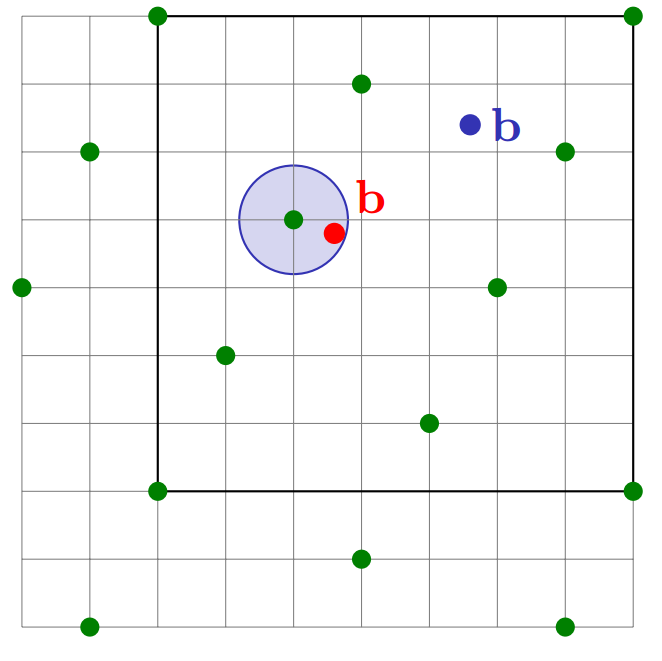
\includegraphics[width=4.5cm]{average-case-bdd}
\caption{Visualization of $\mathrm{LWE}$ reduced to Average-case $\mathrm{BDD}$ problem}
\figuresubtitle{$\textbf{b}^{t} \text{ (in red) } = \textbf{s}^{t}\textbf{A} + \textbf{e}^{t}$ vs. $\textbf{b} \gets \mathbb{Z}^m_q$}
\end{figure}



 



\subsection{\texorpdfstring{$\mathrm{LWE}$}{LWE} problem}
Given samples $(x,y = f(x) + \mathrm{e})$ where $x \in {\mathbb{Z}}_{q}^{n}$, $y \in {\mathbb{Z}}_{q}$ and a linear function $f$ such that $f: {\mathbb{Z}}_{q}^{n} \to {\mathbb{Z}}_{q}$, the idea is to find $f$ or close approximation or it knowing that $e$ (error) comes from a some known noise model. 

\begin{definition}
\normalfont
Learning with errors instance $\mathrm{LWE}_{n,q,\chi}$ is parametrized by:

\begin{itemize}
\item $n$ $\in \mathbb{N}$
\item $q$ $\in$ Primes
\item $\chi$, a probability distribution over $\mathbb{Z}/q\mathbb{Z}$
\end{itemize}

$\chi$ is known as the noise distribution and we would like it to generate short elements, i.e. $||e|| \leq B$ with high probability for some bound $B \ll q$, when $e \leftarrow \chi$. In practice, $\chi$ is usually a discrete Gaussian over $\mathbb{Z}$.
\end{definition}


\begin{theorem}
\normalfont
(\cite{Regev:2005:LLE:1060590.1060603}, Theorem 1.1)
Let $n$, $p$ be integers and $\alpha \in (0, 1)$ be such that $\alpha p > 2 \sqrt{n}$. If there exists an efficient algorithm that solves ${\mathrm{LWE}}_{{q,\Psi_{\alpha }}}$ then there exists an efficient quantum algorithm that approximates the decision version of the shortest vector problem (${\mathrm{GapSVP}}$) and the shortest independent vectors problem (${\mathrm{SIVP}}$) in the worst-case.
\end{theorem}

For the above theorem to work, it is necessary that $\chi$ is chosen to be a discrete Gaussian distribution. This means that sampling from LWE involves taking a lattice point and perturbing it by a small, normally distributed quantity, the idea being that this will look close enough to a uniform distribution if the standard deviation is large enough. Sampling from this discrete Gaussian is simply accomplished by sampling each component from a normal distribution and rounding to the nearest integer.

\subsection{Search \texorpdfstring{$\mathrm{LWE}$}{LWE}}

Suppose we are given an oracle $\mathcal{O}^n_s$ which outputs samples of the form $(a, \langle a, s \rangle + e)$,

\begin{itemize}
\item $\textbf{a} \leftarrow \mathbb{Z}^n_{q}$ is chosen freshly at random for each sample.
\item $\textbf{s} \in \mathbb{Z}^n_{q}$ is the secret (and it is the same for every sample).
\item $\textbf{e} \leftarrow \chi$ is chosen freshly according to $\chi$ for each sample.
\end{itemize}


The search-$\mathrm{LWE}$ problem is to find the secret $\textbf{s}$ given access to $\mathcal{O}^{n}_{\textbf{s}}$. The $\mathrm{LWE}_{n,q,\chi}$ assumption is the assumption that the search-LWE problem is computationally hard.


The $\mathrm{LWE}$ problem described above is the search version of the problem. In the decision version ($\mathrm{DLWE}$), the goal is to distinguish between noisy inner products and uniformly random samples (practically, some discretized version of it). Regev \cite{Regev:2005:LLE:1060590.1060603} showed that the decision and search versions are equivalent when $q$ is a prime bounded by some polynomial in $n$.


\begin{equation}
\centering
\begin{split}
14s_1 + 15s_2 + 5s_3 + 2s_4 \approx 8 \bmod 17\\
13s_1 + 14s_2 + 14s_3 + 6s_4 \approx 16 \bmod 17\\
6s_1 + 10s_2 + 13s_3 + 1s_4 \approx 3 \bmod 17\\
10s_1 + 4s_2 + 12s_3 + 16s_4 \approx 12 \bmod 17\\
9s_1 + 5s_2 + 9s_3 + 6s_4 \approx 9 \bmod 17\\
3s_1 + 6s_2 + 4s_3 + 5s_4 \approx 16 \bmod 17\\
\dots\quad\quad\quad\quad\quad\quad\\
6s_1 + 7s_2 + 16s_3 + 2s_4 \approx 3 \bmod 17
\end{split}
\end{equation}


The $\mathrm{LWE}$ problem asks to recover a secret $ \in \mathbb{Z}^{n}_{q}$ given a sequence of approximate random linear equations on $s$. For instance, the input might be above where each equation is correct up to some small additive error (say, $\{1,-1\}$), and our goal is to recover $\textbf{s}$ (answer in this case is $\textbf{s} = (0, 13, 9, 11)$).


In definition of $\mathrm{LWE}$, error $\textbf{e}$ should be \quotes{short}. Short just means small (in terms of some metric, usually Euclidean norm). We can see that if $\textbf{e}$ is the zero vector, $\textbf{s}$ becomes trivial to recover using Gaussian elimination. If $\textbf{e}$ is uniformly random, then you can imagine that it is impossible to recover any information on $\textbf{s}$, since it is hidden against a uniformly random backdrop. It might be helpful to picture the following instead. Consider $\mathrm{LWE}$ as a lattice, if the vector $\textbf{e}$ is small enough, $\textbf{b}$ is close to only one of the points in this lattice. In other words, the $\mathrm{LWE}$ problem becomes a bounded-distance decoding problem on this lattice. If $\textbf{e}$ is too large, $\textbf{b}$ might be closer to another vector in this lattice. Since we are typically interested in recovering $\textbf{s}$ and not a set of possible secrets, we must be given a guarantee that $\textbf{e}$ is sufficiently short (hence bounded distance decoding).

So \quotes{short} just means that $\textbf{s}$ is recoverable. Usually, $\textbf{e}$ is sampled from a discrete distribution approximating a Gaussian centered around $0$, with small width relative to $q$. This allows one to ensure that $\textbf{s}$ is recoverable with an arbitrarily high probability, while still making the problem as difficult as possible.




\subsection{Ring-\texorpdfstring{$\mathrm{LWE}$}{LWE} Problem}
Adding more structure by considering ideal lattices instead of random ones, we obtain the Ring-$\mathrm{LWE}$ problem, also called the RLWE problem.

Let $n \in \mathbb{N}$ be a power of two, $R_{q}$ the ring $\mathbb{Z}_{q}[x]/(x^n + 1)$ for a positive integer $q$ and $\chi_{\sigma}$ the corresponding ($n$-dimensional) error distribution on $R_{q}$. Given $R_{q}$, $s$, $a \in R_{q}$ and $e \leftarrow \chi_{\sigma}$, we define $A_{s, \chi_{\sigma}}$ to be the distribution of the resulting pairs $(a, a s + e) \in R_{q} \times R_{q}$.


\textbf{The RLWE$_{q,\sigma}$ Assumption}:  the assumption states that it is hard for any polynomial time algorithm with only polynomially many samples to distinguish $A_{s,\chi_{\sigma}}$ from the uniform distribution on $R_q \times R_q$.

Regev in \cite{cryptoeprint:2012:230} proved that there exists a probabilistic polynomial-time quantum algorithm that reduces approximate $\mathrm{S(I)VP}$ in the worst-case to average-case decision-$\mathrm{RLWE}$. This reduction proves the hardness of RLWE.

% Let $K$ be the $m$th cyclotomic number field having degree $n = \phi(m)$ and $\mathcal{O}_{K}$ be its ring of integers. Let $\alpha < \sqrt{\log n}$, and let $q = q(n) \ge 2$, $q = 1 \bmod m$ be a $poly(n)$-bounded prime such that $\alpha q \ge \omega(\sqrt{\log n})$. Then there is a polynomial-time quantum reduction from $\mathcal{O}(\sqrt{n} / \alpha)$-approximate $\mathrm{SIVP}$ (of $\mathrm{SVP}$) on ideal lattices in $K$ to decision-RLWE$_q$. Alternatively, for any $l \ge 1$, we can replace the target problem of solving decision-RLWE$_q$ given only $l$ samples.

The $\mathrm{RLWE}$ problem can be stated in two different ways: a \quotes{search} version and a \quotes{decision} version. Both begin with the same construction. Let:

\begin{itemize}
    \item $a_{i}(x)$ be a random element but known polynomials from $\mathbb{Z} _{q}[x]/ (\Phi (x))$ with coefficients from all of $\mathbb{Z}_q$
    
    \item $e_{i}(x)$ be small random element and unknown polynomials relative to a bound $b$ in the ring $\mathbb {Z} _{q}[x]/ (\Phi (x))$
    
    \item $s(x)$ be a small unknown polynomial relative to a bound $b$ in the ring $\mathbb{Z}_{q}[x]/ (\Phi (x))$.
    
    \item $b_{i}(x)=(a_{i}(x)\cdot s(x))+e_{i}(x)$
\end{itemize}


The Search version entails finding the unknown polynomial $s(x)$ given the list of polynomial pairs $(a_{i}(x),b_{i}(x))$.

The Decision version of the problem can be stated as follows. Given a list of polynomial pairs $(a_{i}(x),b_{i}(x))$, determine whether the $b_{i}(x)$ polynomials were constructed as $b_{i}(x)=(a_{i}(x)\cdot s(x))+e_{i}(x)$ or were generated randomly from $\mathbb{Z} _{q}[x]/(\Phi (x))$ with coefficients from all of $\mathbb{Z}_q$.

The difficulty of this problem is parametrized by the choice of the quotient polynomial ($\Phi (x)$), its degree ($n$), the field ($\mathbb{Z}_q$), and the smallness bound ($b$). In many $\mathrm{R\text{-}LWE}$ based public key algorithms the private key will be a pair of small polynomials $s(x)$ and $e(x)$. The corresponding public key will be a pair of polynomials $a(x)$, selected randomly from $\mathbb{Z} _{q}[x]/(\Phi (x))$, and the polynomial $t(x)=(a(x)\cdot s(x))+e(x)$. Given $a(x)$ and $t(x)$, it should be computationally infeasible to recover the polynomial $s(x)$.


% \subsection{How to generate new \texorpdfstring{$\mathrm{LWE}$}{LWE} samples}
% The basic idea is to take random (Gaussian) integer combinations of the given $\mathrm{LWE}$ samples, and add a little \textit{smoothing} noise. This will result in new samples which are statistically close to $\mathrm{LWE}$ samples with the same secret, but with a somewhat wider error distribution (by a factor of $\tilde{O}(\sqrt{n})$ for typical parameters).

% More precisely, given $\mathrm{LWE}$ samples grouped as $\mathbf{A} \in \mathbb{Z}_q^{n \times m}, \mathbf{b}^t = \mathbf{s}^t \mathbf{A} + \mathbf{e}^t$ where $m \approx n \log q$, generate a new sample as $\mathbf{a}' = \mathbf{A} \cdot \mathbf{r} \in \mathbb{Z}_q^n, b' = \mathbf{b}^t \cdot \mathbf{r} + \tilde{e} \in \mathbb{Z}_q$, where $\mathbf{r} \in \mathbb{Z}^m$ and $\tilde{e} \in \mathbb{Z}$ have discrete Gaussian distributions of appropriate parameters.  One can show that with high probability over the choice of the original $(\mathbf{A}, \mathbf{b})$, the distribution of $\mathbf{a}'$ is nearly uniform. Moreover, conditioned on any fixed choice of $\mathbf{a}'$, the distribution of $\mathbf{e}^t \cdot \mathbf{r} + \tilde{e}$ (which is the \quotes{error} term in the output sample) is close to a discrete Gaussian.

% The $\mathrm{LWE}$ dimension here is $n$, and is preserved by the process we just described. The original $(\textbf{A},\textbf{b}')$ corresponds to $m$ LWE samples (one for each column of $\textbf{A}$), where the secret has dimension $n$. The above process generates a fresh sample having exactly the same $n$-dimensional secret. We can of course run the method an unbounded number of times to get as many new samples as we want. This procedure is described in Gentry-Peikert-Vaikuntanathan, \textit{Trapdoors for Hard Lattices} \cite{Gentry:2008:THL:1374376.1374407}



\begin{figure}[H]
\centering
\iftoggle{verylong}{
\lstinputlisting[language=Python]{code_snippets/gaussian_sampler_plot.sage}
}{}

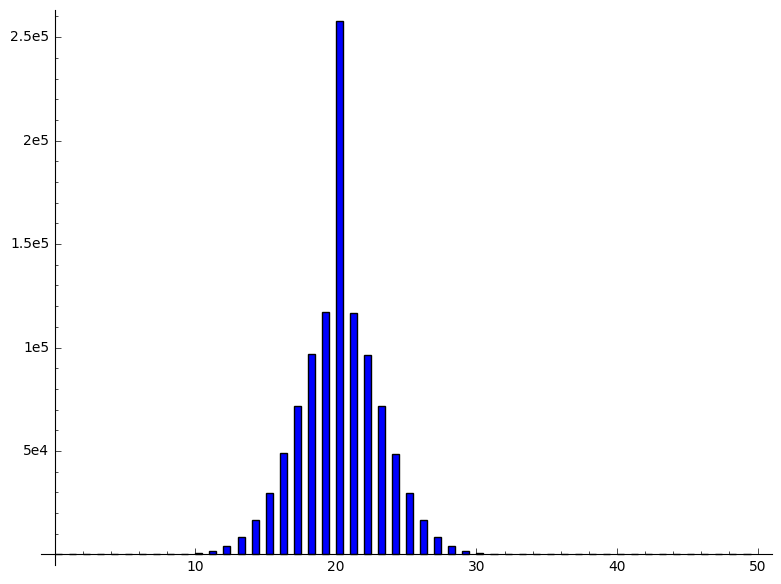
\includegraphics[scale=0.3]{gaussian_distribution}
\caption{Plot of Gaussian distribution centered at $20$, $\sigma = \frac{8}{\sqrt{2  \pi}}$}
\end{figure}
